\documentclass[11pt]{article}

\usepackage[T1]{fontenc}
\usepackage[utf8]{inputenc}
\usepackage[a4paper,margin=1in]{geometry}
\usepackage{amsmath,amssymb}
\usepackage{graphicx}
\usepackage{booktabs}
\usepackage{xcolor}
\usepackage{caption}
\usepackage{listings}
\usepackage{mdframed}
\usepackage[authoryear,round]{natbib}
\usepackage[colorlinks=true,linkcolor=blue!50!black,citecolor=blue!50!black,urlcolor=blue!50!black]{hyperref}

\definecolor{codebg}{gray}{0.96}
\definecolor{codekw}{rgb}{0.0,0.3,0.6}
\definecolor{codecm}{rgb}{0.3,0.5,0.3}
\lstset{
  basicstyle=\ttfamily\small,
  backgroundcolor=\color{codebg},
  keywordstyle=\color{codekw}\bfseries,
  commentstyle=\color{codecm}\itshape,
  breaklines=true, showstringspaces=false, frame=single, framesep=4pt,
  language=Python, columns=fullflexible,
}
\newmdenv[linecolor=blue!40!black,linewidth=0.8pt,backgroundcolor=blue!3,
          skipabove=8pt,skipbelow=8pt,innertopmargin=6pt,innerbottommargin=6pt]{keybox}
\newmdenv[linecolor=orange!60!black,linewidth=0.8pt,backgroundcolor=orange!5,
          skipabove=8pt,skipbelow=8pt,innertopmargin=6pt,innerbottommargin=6pt]{warnbox}

\newcommand{\E}{\mathbb{E}}
\newcommand{\R}{\mathbb{R}}
\newcommand{\code}[1]{\texttt{#1}}
\newcommand{\flm}{f_{\ell m}}

\title{\textbf{The \code{gfs\_dynamical\_core.jax} Technical Manual}\\[4pt]
\large A differentiable spectral primitive-equation dynamical core in JAX}
\author{\code{gfs\_dynamical\_core} / \code{docs/gfs\_jax\_manual/}}
\date{\today}

\begin{document}
\maketitle

\begin{abstract}
\noindent
\code{gfs\_dynamical\_core.jax} is a dry, spectral, primitive-equation atmospheric
dynamical core --- a re-implementation of the hydrostatic GFS/SHTNS Fortran core ---
written entirely as pure \code{JAX} functions. Because every operation is a
traceable \code{JAX} primitive, the whole model is \code{jit}-compilable,
\code{vmap}-vectorisable over ensembles, and, above all, \emph{differentiable}:
one can take exact derivatives of any forecast quantity with respect to the
initial state, the parameters, or the forcing, in either reverse (adjoint) or
forward (tangent-linear) mode, without writing a separate adjoint model. This
manual documents the architecture and numerics of the core, shows how to build
and run a Held--Suarez model on top of it, and --- the main event --- explains
what differentiability buys you and how to use it, with six short, runnable
example scripts (sensitivities, Jacobians, ensembles, variational optimisation,
singular vectors). It is written for a graduate student or research scientist who
knows atmospheric dynamics and some Python, and wants to \emph{use} the core, not
just read about it.
\end{abstract}

\tableofcontents
\newpage

%==============================================================================
\part{The dynamical core}
%==============================================================================

\section{Introduction and scope}

The core solves the \textbf{dry hydrostatic primitive equations} on the sphere in
\textbf{spherical-harmonic (spectral) space}, on a hybrid sigma--pressure vertical
coordinate, with a semi-implicit IMEX Runge--Kutta time scheme. It is a faithful
port of an operational-lineage Fortran core (GFS dynamics, SHTNS transforms): the
numerics --- the vertical discretisation, the semi-implicit gravity-wave treatment,
the hyper-diffusion, the dry-mass fixer --- are reproduced, and validated against
the Fortran reference. What is new is the \emph{substrate}: the code is pure
\code{JAX}, so it inherits automatic differentiation, JIT compilation, and
vectorisation.

\begin{keybox}
\textbf{Why re-write a working Fortran core in JAX?} Not for raw speed (on CPU it
is comparable). The payoff is \emph{composability with autodiff and hardware
acceleration}: gradients of a forecast metric with respect to millions of inputs
at the cost of a single extra integration (\S\ref{sec:diff}); ensembles as a
batch axis (\S\ref{sec:vmap}); and the ability to embed the core inside a larger
differentiable program (a machine-learned parametrisation, a variational
assimilation, an optimisation loop) and train the whole thing end-to-end. None of
these are available from a conventional Fortran core without writing and
maintaining separate tangent-linear and adjoint models by hand.
\end{keybox}

The core is deliberately \emph{small} and readable: four modules, $\sim$1800 lines
(Table~\ref{tab:modules}).

\begin{table}[h]
\centering
\caption{The four modules of \code{gfs\_dynamical\_core.jax}.}
\label{tab:modules}
\begin{tabular}{lp{10.5cm}}
\toprule
module & responsibility \\
\midrule
\code{states.py} & the state containers (\code{SpectralState}, \code{GridState},
  \code{GridGradients}, \code{SpectralTendencies}) as \code{flax} pytrees. \\
\code{transforms.py} & spherical-harmonic transforms (scalar and spin-weighted),
  precompute-kernel caching, grid geometry, triangular-truncation \& reality
  enforcement. \\
\code{dynamics.py} & the primitive-equation right-hand side: pressure diagnostics,
  vertical velocities, pressure-gradient force, vertical advection, energy
  conversion, tendency assembly, dry-mass fixer. \\
\code{stepper.py} & time integration: the 3-stage IMEX-RK scheme, the
  semi-implicit gravity-wave solve, hyper-diffusion/Rayleigh damping, and the
  physics-injection entry point \code{advance\_with\_tendencies}. \\
\bottomrule
\end{tabular}
\end{table}

\section{Architecture and data flow}\label{sec:arch}

One model time step is a loop through spectral and grid space:
\begin{enumerate}
\item Start from the \textbf{spectral state} $S$ (vorticity, divergence,
  temperature, $\ln p_s$, tracers --- as spherical-harmonic coefficients).
\item \textbf{Inverse transform} $S\to$ grid state $G$ (winds $u,v$, temperature,
  $\ln p_s$, tracers) \emph{and} the horizontal gradients needed by the dynamics
  (\code{spectral\_to\_grid}).
\item Evaluate the nonlinear \textbf{primitive-equation tendencies} in grid space
  (\code{full\_dynamics\_step}): products like $u\,\zeta$, the pressure-gradient
  force, vertical advection --- everything that is cheap and local on the grid.
\item \textbf{Forward transform} the grid tendencies back to spectral tendencies
  (\code{grid\_to\_spectral\_tendencies}), where the linear terms (Laplacians,
  gravity waves) are diagonal and cheap.
\item \textbf{Advance} in spectral space with the semi-implicit IMEX-RK scheme,
  apply diffusion, optionally inject physics (\code{advance}).
\end{enumerate}
The grid $\leftrightarrow$ spectral round trip per stage is the defining feature
of a spectral transform model: nonlinear products are done where they are local
(grid), linear operators where they are diagonal (spectral). The core does this
three times per step (a 3-stage RK).

\section{Environment and conventions}\label{sec:conventions}

\begin{keybox}
\textbf{Float64 is mandatory; pin the CPU backend on Apple Silicon.} The spectral
dynamics are numerically stiff and single precision corrupts them silently. Set,
\emph{before importing \code{jax}}:
\begin{lstlisting}
import os
os.environ["JAX_ENABLE_X64"] = "True"
os.environ.setdefault("JAX_PLATFORMS", "cpu")  # Metal (Apple GPU) has no float64
\end{lstlisting}
A cluster exporting \code{JAX\_PLATFORMS=cuda} still wins (note the
\code{setdefault}). Getting this wrong gives either a crash or, worse, quietly
degraded numbers.
\end{keybox}

\paragraph{Vertical indexing: bottom-to-top.} Level index $k=0$ is the surface,
$k=n_{\text{lev}}$ the model top. All fields, coordinate coefficients \code{ak/bk},
and diagnostics use this convention. (The Fortran reference is top-to-bottom in
places; the port standardises on bottom-to-top and the semi-implicit setup flips
internally.)

\paragraph{Grid geometry.} Gauss--Legendre (GL) sampling: $n_{\text{lat}}=L$,
$n_{\text{lon}}=2L-1$, where $L$ is the spherical-harmonic band-limit. Latitudes
are Gaussian quadrature points, north-to-south. The \emph{physical} triangular
truncation $T$ (de-aliasing) defaults to the GFS convention
$T=\lfloor n_{\text{lon}}/3-2\rfloor$; spectral arrays are stored on the full
$(L,\,2L-1)$ rectangle but coefficients with $\ell>T$ or $|m|>T$ are zeroed after
every forward transform.

\paragraph{Setup-time constants come from \code{climt}.} The vertical coordinate
(\code{ak},\code{bk}) and Earth constants ($R_d$, $c_p$, $\Omega$, $g$, radius,
model-top pressure) are fetched once from \code{climt.get\_grid(...)} at build time
(\S\ref{sec:build}). Nothing in the time loop depends on \code{climt}.

\section{State representation}\label{sec:states}

States are \code{flax.struct} dataclasses --- i.e.\ JAX \emph{pytrees}: their array
fields are traced leaves (so \code{jit}/\code{grad}/\code{vmap} see through them),
while scalar configuration fields can be marked static. The two central containers
(\code{states.py}):

\begin{lstlisting}
@struct.dataclass
class SpectralState:            # spherical-harmonic coefficients (complex128)
    vorticity:            # (n_lev, L, 2L-1)
    divergence:           # (n_lev, L, 2L-1)
    temperature:          # (n_lev, L, 2L-1)
    log_surface_pressure: # (L, 2L-1)
    tracers:              # (n_tracers, n_lev, L, 2L-1)

@struct.dataclass
class GridState:                # physical fields on the Gaussian grid (float64)
    u, v, temperature, vorticity, divergence:  # (n_lev, n_lat, n_lon)
    log_surface_pressure:                       # (n_lat, n_lon)
    tracers:                                    # (n_tracers, n_lev, n_lat, n_lon)
\end{lstlisting}

The prognostic variables are the \emph{vorticity--divergence} form of the momentum
equations (not $u,v$): this makes the linear terms diagonal in spectral space.
\code{GridGradients} carries the horizontal derivatives of $\ln p_s$, temperature
and tracers (produced for free by the spin-weighted transform, \S\ref{sec:transforms});
\code{SpectralTendencies} mirrors \code{SpectralState} with $\partial/\partial t$
of each field. Because states are pytrees, an ``ensemble of states'' is just the
same pytree with a leading batch axis, and a ``perturbation to a state'' is a
pytree of the same shape --- both facts we lean on heavily in Part III.

\section{Spectral transforms}\label{sec:transforms}

The transforms (\code{transforms.py}) are built on \code{s2fft}. Three points
matter for a user.

\paragraph{Scalar and spin-weighted transforms.} Temperature, $\ln p_s$ and
tracers are ordinary scalar fields (spin-0). The winds are handled with
\textbf{spin-1} transforms: from vorticity $\zeta$ and divergence $D$,
\begin{equation}
  F^{(1)}_{\ell m} = \frac{R}{\sqrt{\ell(\ell+1)}}\,(D_{\ell m} + i\zeta_{\ell m}),
  \qquad u = \operatorname{Im} f^{(1)},\quad v = -\operatorname{Re} f^{(1)},
\end{equation}
and inversely, \code{grid\_to\_spectral} uses \emph{both} spin $+1$ and spin $-1$
forward transforms to recover $D_{\ell m}$ and $\zeta_{\ell m}$ exactly for all
$m$ (a single transform loses information for $m\ge 1$, where $D,\zeta$ are
complex). The same spin-1 machinery yields the horizontal \emph{gradients} of
scalars (temperature, $\ln p_s$) as a by-product, which the pressure-gradient and
advection terms need.

\paragraph{Precompute kernels.} \code{s2fft}'s on-the-fly Wigner recursions
dominate cost ($\sim$7\,ms/transform at $L=64$). The core instead uses
\emph{precompute kernels} --- each transform becomes a dense contraction
($\sim$0.6\,ms, $\sim$12$\times$ faster, matching the recursions to $\sim$$10^{-12}$).
Kernels are cached per $(L,\text{sampling},\text{spin},\text{direction})$ and,
under \code{jit}, are baked in as constants. Kernel construction is \emph{not}
\code{jit}-traceable, so it must happen eagerly \emph{before} tracing:
\begin{lstlisting}
from gfs_dynamical_core.jax.transforms import prebuild_kernels
prebuild_kernels(L, "gl")   # call once at setup, before any jit-compiled step
\end{lstlisting}

\paragraph{Triangular truncation and the reality condition.} After every forward
transform, \code{enforce\_triangular\_truncation} (i) zeroes coefficients with
$\ell>T$ or $|m|>T$, and (ii) enforces the reality condition
$f_{\ell,-m}=(-1)^m\overline{f_{\ell,+m}}$ with $\operatorname{Im}f_{\ell,0}=0$.

\begin{keybox}
\textbf{Why the reality condition is not optional.} \code{s2fft} stores the full
$(\ell,\pm m)$ rectangle and treats fields as \emph{general complex} functions.
Round-off (mainly in the dual-spin forward combinations) seeds a tiny violation of
$f_{\ell,-m}=(-1)^m\overline{f_{\ell,+m}}$ --- which \emph{is} an imaginary-valued
grid field. That imaginary field evolves as an \emph{undamped tangent-linear
perturbation} of the flow: it e-folds with the jet's fastest instability
($\sim$5.5\,h) and, coupling back through the nonlinear terms, blows the model up
around day 7--8. SHTNS/Fortran store only $m\ge 0$ and so are symmetric by
construction; enforcing the symmetry at every forward transform makes the JAX core
do the same, and all subsequent real-coefficient linear operations preserve it.
This was one of the subtle bugs found and fixed during the port.
\end{keybox}

\section{The primitive-equation dynamics}\label{sec:dynamics}

\code{dynamics.py} evaluates the right-hand side. On the hybrid coordinate the
interface pressures are $p_k = a_k + b_k(p_s - p_{\text{top}})$
(\code{compute\_pressure\_diagnostics}), from which layer thicknesses $\Delta p$,
layer-mean pressures, and the geometric factors $\alpha,\ \delta\!\ln p$ follow.
The pipeline (\code{full\_dynamics\_step}) is:

\begin{enumerate}
\item \textbf{Vertical velocities} (\code{compute\_vertical\_velocities}): vertically
  integrate the continuity equation to get the surface-pressure tendency
  $\partial_t\ln p_s$, the coordinate vertical velocity $\dot\eta$ on interfaces,
  and $\omega=\mathrm{d}\ln p/\mathrm{d}t$ on layers.
\item \textbf{Pressure-gradient force} (\code{compute\_pressure\_gradient\_force}):
  the horizontal PGF from virtual temperature, $\ln p_s$ gradients and the
  surface-geopotential gradients, integrated through the hybrid layers.
\item \textbf{Vertical advection}: second-order centred for $u,v,T$
  (\code{compute\_vertical\_advection}); a positive-definite \citet{thuburn1996}
  flux-limited scheme for tracers (\code{compute\_vertical\_advection\_tracers}) so
  that mixing ratios cannot go negative.
\item \textbf{Energy conversion} $\kappa\,\omega\,T_v/[1+(c_{vap}/c_p-1)q]$.
\item \textbf{Assemble tendencies} (\code{assemble\_grid\_tendencies}): the flux form
  $u\text{-flux}=u(\zeta+f)+(\text{vadv}_v-\text{PGF}_y)$ etc.\ with Coriolis
  $f=2\Omega\sin\phi$, temperature and tracer tendencies, and kinetic energy.
\end{enumerate}
\code{grid\_to\_spectral\_tendencies} then maps these back: $\partial_t\zeta =
-\nabla\!\cdot\text{flux}$, $\partial_t D = \nabla\times\text{flux} -
\nabla^2(\text{KE})$. Optionally a \textbf{dry-mass fixer}
(\code{compute\_dry\_mass\_fixer}) rescales the $\ln p_s$ tendency each step so the
global dry-air mass is conserved.

\section{Time integration}\label{sec:stepper}

The stepper (\code{stepper.py}) is a \textbf{3-stage IMEX Runge--Kutta} scheme: the
fast linear gravity-wave terms are treated \emph{implicitly} (so the time step is
not limited by the sound/gravity-wave speed), the nonlinear advective terms
\emph{explicitly}.

\paragraph{Semi-implicit gravity-wave solve.} The gravity-wave terms are linearised
about a reference state ($T_{\text{ref}}=300$\,K, $p_{s,\text{ref}}=800$\,hPa),
giving four wavenumber-independent operators built once by
\code{init\_semi\_implicit\_matrices}: \code{amhyb} (geopotential PGF acting on
$T_v$), \code{bmhyb} (energy conversion acting on $D$), \code{tor\_hyb} ($\ln p_s$
in the PGF) and \code{svhyb} ($\ln p_s$ tendency from $D$). With
$Y_m=\text{tor\_hyb}\otimes\text{svhyb}+\text{amhyb}\cdot\text{bmhyb}$ the implicit
solve at each stage and each degree $\ell$ inverts
\begin{equation}
  \bigl(I + (c\,\Delta t)^2\,\ell(\ell+1)\,Y_m\bigr)^{-1},
\end{equation}
pre-computed as \code{d\_hyb\_m} of shape $(3, L, n_{\text{lev}}, n_{\text{lev}})$
(three implicit coefficients $c$, one $n_{\text{lev}}\times n_{\text{lev}}$
inverse per degree). Vorticity and tracers are advanced explicitly; divergence,
temperature and $\ln p_s$ go through the implicit solve.

\paragraph{Diffusion.} \code{init\_diffusion\_operators} builds a spectral
hyper-diffusion operator $\propto[\ell(\ell+1)/\ell_{\max}(\ell_{\max}+1)]^{4}$
($\nabla^8$, \code{ndiss}=8), a height-dependent enhancement profile, and an
optional upper-level Rayleigh damping. These are applied as an implicit linear
factor at the end of each step.

\paragraph{The two entry points.} \code{advance(...)} performs one dynamics-only
step. \code{advance\_with\_tendencies(...)} performs the same dynamics step and
then applies a \emph{time-split physics increment}:
\begin{lstlisting}
advance_with_tendencies(spec_state, phys_tends, phis_grads, dyn_config,
                        trans_config, stepper_config, latitudes,
                        gauss_weights=None, pdryini=None, spec_tends=None)
\end{lstlisting}
\code{phys\_tends} is a grid-space \code{PhysicsTendencies} (e.g.\ Held--Suarez
forcing, or a machine-learned parametrisation) transformed to spectral internally;
\code{spec\_tends} is a spectral-space increment added \emph{directly} (the
injection point for stochastic schemes such as SPPT/SKEB). With both \code{None}
it is exactly \code{advance}. The increment is applied as
$S_{\text{new}} = S_{\text{dyn}} + \Delta t\,(\text{increment})$.

%==============================================================================
\part{Building and running a model}
%==============================================================================

\section{Building a Held--Suarez model}\label{sec:build}

The core provides the dynamics; a \emph{model} adds a vertical coordinate,
constants, and a forcing. The reference builder is
\code{docs/gfs\_jax\_manual/examples/\_model.py}. It (i) fetches \code{ak,bk} and
Earth constants from \code{climt}; (ii) assembles the \code{DynamicsConfig},
\code{TransformConfig}; (iii) pre-builds transform kernels; (iv) builds the
semi-implicit and diffusion operators; and (v) packs everything into a single
pytree \code{ModelBundle}:

\begin{lstlisting}
bundle = build_model("T21")          # L=32, T=21, dt=1800 s, 20 levels
# ModelBundle carries: dyn_config, trans_config, stepper_config, latitudes,
# gauss_weights, phis_grads, dt, n_lev.  Array leaves are differentiable;
# dt / n_lev are static pytree aux, so one jit graph is reused across steps.
\end{lstlisting}

A single deterministic step is then just the grid$\to$tendency$\to$advance
sequence:
\begin{lstlisting}
def step(bundle, spec_state):
    grid, _ = spectral_to_grid(spec_state, bundle.trans_config)
    phys = hs_tendencies(grid, bundle)                 # Held-Suarez forcing
    return advance_with_tendencies(
        spec_state, phys, bundle.phis_grads, bundle.dyn_config,
        bundle.trans_config, bundle.stepper_config, bundle.latitudes,
        bundle.gauss_weights, None)
\end{lstlisting}

\section{The Held--Suarez forcing}

\citet{heldsuarez1994} is the standard idealised forcing for testing dynamical
cores: Newtonian relaxation of temperature towards a prescribed radiative
equilibrium $T_{\text{eq}}(\phi,p)$ at a latitude/height-dependent rate, plus
Rayleigh friction of low-level winds. It has no moisture and no radiation code, so
it is cheap, reproducible, and isolates the dynamics. In the core's terms it is
just a function \code{hs\_tendencies(grid\_state, bundle)} returning a
\code{PhysicsTendencies}; swapping in a different (even machine-learned) physics is
a matter of returning the same container.

\section{Integrating in time with \code{lax.scan}}\label{sec:scan}

Do \emph{not} write a Python \code{for} loop over steps: it would unroll into a
giant graph. The idiomatic long integration is a \code{jax.lax.scan}, compiled once
with \code{jax.jit}:
\begin{lstlisting}
@partial(jax.jit, static_argnums=(2,))
def run(bundle, spec0, n_steps):
    def body(spec, _):
        spec = step(bundle, spec)
        # ... optionally compute and stack a diagnostic here ...
        return spec, diagnostic
    spec_final, trace = jax.lax.scan(body, spec0, None, length=n_steps)
    return spec_final, trace
\end{lstlisting}
This is \textbf{Example 1} (\code{ex01\_run\_forward.py}): a 6-day Held--Suarez
spin-up from an isothermal rest state, watching kinetic energy grow as the jet and
baroclinic eddies develop (Figure~\ref{fig:spinup}). For very long or memory-heavy
integrations, wrap \code{body} in \code{jax.checkpoint} to trade compute for memory
(\S\ref{sec:caveats}).

\begin{figure}[h]
\centering
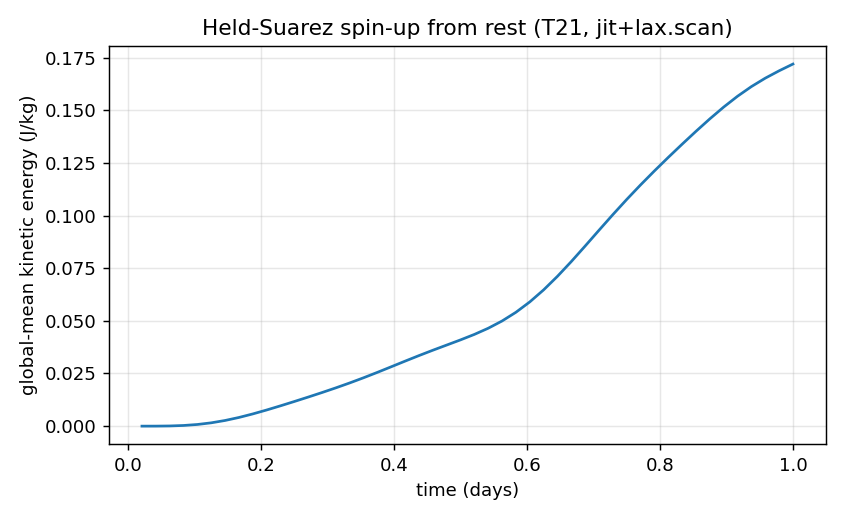
\includegraphics[width=0.62\textwidth]{figures/fig_spinup.png}
\caption{Example 1: global-mean kinetic energy during a Held--Suarez spin-up from
rest (T21), computed by a single \code{jit}-compiled \code{lax.scan}.}
\label{fig:spinup}
\end{figure}

%==============================================================================
\part{Differentiable modelling}
%==============================================================================

\section{What differentiability buys a GCM}\label{sec:diff}

Every quantity the core computes is a composition of differentiable \code{JAX}
primitives. Consequently any scalar \emph{metric} $J$ of a forecast --- a global
mean, a regional average, a misfit to observations, a forecast error --- is a
differentiable function of whatever it depends on: the initial state $x_0$, the
model parameters $\theta$, the forcing. \code{JAX} gives the derivatives exactly
(to machine precision, not by finite differences) and cheaply.

\begin{keybox}
\textbf{The adjoint, for free.} In a conventional GCM, obtaining
$\partial J/\partial x_0$ (the sensitivity of a forecast metric to the initial
state) requires a hand-written \emph{adjoint model}: a separate code, derived
line-by-line from the forward model, that must be re-derived and re-validated every
time the forward model changes. It is one of the most labour-intensive artefacts in
numerical weather prediction. Here it is one function call, \code{jax.grad(J)},
generated automatically from the forward code and therefore \emph{always}
consistent with it. The tangent-linear model is likewise \code{jax.jvp}; the
adjoint is \code{jax.vjp}.
\end{keybox}

\subsection{What the gradient is, and with respect to what}

Let $J:\;\mathcal X\to\R$ map an input (an initial-state field, a vector of
parameters, \dots) to a scalar. \code{jax.grad(J)(x)} returns
$\nabla_x J$, an object of the \emph{same pytree shape as $x$} --- e.g.\ if $x$ is
an initial temperature field of shape $(n_{\text{lev}},n_{\text{lat}},n_{\text{lon}})$,
then $\nabla_x J$ is a field of that shape whose value at each point says how much
$J$ changes per unit change of the initial temperature there. The gradient is
taken with respect to \emph{whatever you pass as the differentiated argument}, and
nothing else is moved.

\subsection{Reverse mode vs.\ forward mode}

For a map $f:\R^n\to\R^m$ autodiff comes in two flavours:
\begin{itemize}
\item \textbf{Reverse mode} (\code{grad}, \code{jacrev}, \code{vjp}) propagates
  \emph{cotangents} backwards. Cost $\propto m$ (number of outputs). Use it when
  outputs are few and inputs many --- the usual case $m=1$ (a scalar metric, so one
  backward pass gives the full gradient over all $n$ inputs). This is the adjoint.
\item \textbf{Forward mode} (\code{jacfwd}, \code{jvp}) propagates \emph{tangents}
  forwards. Cost $\propto n$ (number of inputs). Use it when inputs are few and
  outputs many. This is the tangent-linear model.
\end{itemize}
A full Jacobian is $\min(m,n)$ such passes; \code{jax.jacrev} and \code{jax.jacfwd}
build it for you and agree to rounding (Example~4).

\section{Six capabilities, six scripts}\label{sec:examples}

Each script lives in \code{docs/gfs\_jax\_manual/examples/} and runs at T21 in a few
minutes on a laptop CPU. Run e.g.\ \code{python -m
docs.gfs\_jax\_manual.examples.ex03\_gradient\_sensitivity}.

\subsection{Example 1 --- forward run (\code{jit} + \code{lax.scan})}
Covered in \S\ref{sec:scan}: compile the whole time loop once and integrate.
The foundation everything else builds on.

\subsection{Example 2 --- ensembles with \code{vmap}}\label{sec:vmap}
A Fortran core runs one state per process; an ensemble means many executables.
Here the model is a pure function of its state, so \code{jax.vmap} vectorises the
\emph{same compiled} integration over a batch of perturbed initial conditions --- the
ensemble is one array axis:
\begin{lstlisting}
ens0 = jax.vmap(perturb)(keys)                          # batched SpectralState
ke   = jax.vmap(lambda s: rollout(bundle, s, n_steps))(ens0)   # one call, all members
\end{lstlisting}
\code{ex02\_ensemble\_vmap.py} launches an 8-member ensemble from tiny
initial-temperature perturbations and shows the members diverging (chaotic growth)
after a couple of days. The same axis could be a batch of \emph{parameter} settings
or \emph{forcings}.

\subsection{Example 3 --- adjoint sensitivity with \code{grad}}
The capability a Fortran core cannot give without a hand-coded adjoint. Define a
scalar forecast metric $J=$ global-mean kinetic energy after 12\,h, as a function
of the \emph{initial temperature field} $T_0$, and compute $\partial J/\partial
T_0$ with one call:
\begin{lstlisting}
J, dJ_dT0 = jax.value_and_grad(metric)(T0)      # the adjoint sensitivity map
\end{lstlisting}
$\partial J/\partial T_0[k,j,i]$ is the change in later kinetic energy per unit
initial-temperature perturbation at each point (Figure~\ref{fig:sens}). This is a
one-integration-cost answer to ``where does the initial state most control this
forecast metric?'' --- the question at the heart of targeted observations,
sensitivity analysis, and data assimilation.

\begin{figure}[h]
\centering
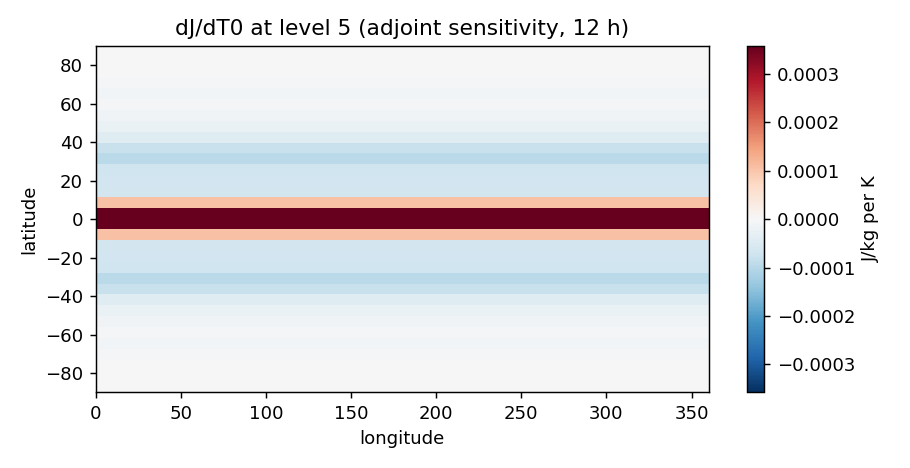
\includegraphics[width=0.75\textwidth]{figures/fig_sensitivity.png}
\caption{Example 3: adjoint sensitivity $\partial J/\partial T_0$ of a 12-hour
kinetic-energy metric to the initial temperature field, at the most sensitive
model level. Structure is near-zonal because the (lightly spun-up) base state is
near-zonally-symmetric; the equatorial band dominates. Produced by
\code{jax.grad}, at the cost of $\sim$one forward integration.}
\label{fig:sens}
\end{figure}

\subsection{Example 4 --- Jacobians (\code{jacfwd} / \code{jacrev})}
For a small vector-to-vector map $f:\R^k\to\R^m$ ($k$ initial-perturbation
amplitudes $\to$ $m$ forecast diagnostics), both modes build the same Jacobian:
\begin{lstlisting}
Jr = jax.jacrev(f)(theta0)     # reverse: cheap when m < k
Jf = jax.jacfwd(f)(theta0)     # forward: cheap when k < m
# max|Jr - Jf| ~ 1e-17   (they agree)
\end{lstlisting}
$\partial f_j/\partial\theta_i$ is the tangent-linear response of diagnostic $j$ to
perturbation $i$ --- a tangent-linear model restricted to a chosen
input/output subspace. \code{ex04\_jacobian.py} prints the $3\times 4$ matrix and
verifies forward/reverse agreement.

\subsection{Example 5 --- variational optimisation (a 4D-Var flavour)}
Because the forecast is differentiable end-to-end, one can \emph{fit} the initial
state (or parameters) so a forecast matches a target --- the essence of 4D-Var and
of parameter estimation. \code{ex05\_optimize\_ic.py} adjusts a few
initial-temperature amplitudes by gradient descent so the forecast kinetic energy
hits a prescribed target (Figure~\ref{fig:opt}):
\begin{lstlisting}
loss_and_grad = jax.jit(jax.value_and_grad(lambda th: (ke_of(th) - target)**2))
for it in range(steps):
    loss, g = loss_and_grad(theta)
    theta = theta - lr * g / (jnp.linalg.norm(g) + 1e-12)
\end{lstlisting}
Swap the metric for an observation-misfit plus a background term and this is
variational data assimilation; swap $\theta$ for physics parameters and it is
gradient-based calibration.

\begin{figure}[h]
\centering
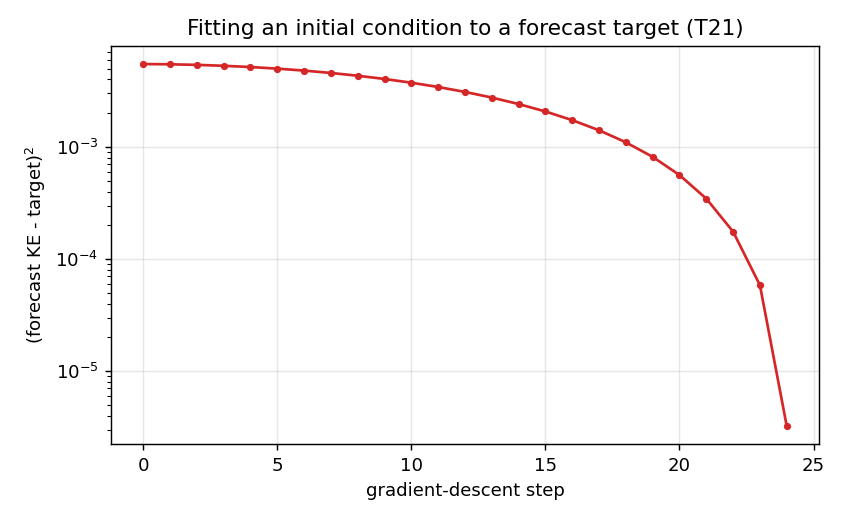
\includegraphics[width=0.6\textwidth]{figures/fig_optimize.png}
\caption{Example 5: gradient descent through the model fits an initial condition so
that the forecast kinetic energy reaches a target (squared misfit vs.\ iteration).}
\label{fig:opt}
\end{figure}

\subsection{Example 6 --- optimal perturbations / singular vectors (\code{jvp}+\code{vjp})}
The tangent-linear propagator $M=\partial(\text{rollout})/\partial x$ and its
adjoint $M^\top$ are exactly \code{jax.jvp} and \code{jax.vjp}. The leading
\emph{singular vector} --- the initial perturbation that grows fastest over a window,
central to predictability and ensemble design --- is the top eigenvector of
$M^\top M$, found by power iteration using only these two:
\begin{lstlisting}
_, vjp_fn = jax.vjp(g, x0)                     # adjoint  M^T
apply_M   = lambda dx: jax.jvp(g, (x0,), (dx,))[1]   # tangent-linear  M
dx = random_unit_vector
for _ in range(iters):
    Mdx = apply_M(dx); growth = norm(Mdx)      # ||M dx|| with ||dx|| = 1
    dx  = vjp_fn(Mdx)[0]; dx = dx / norm(dx)   # dx <- M^T M dx, renormalise
\end{lstlisting}
\code{ex06\_singular\_vector.py} converges to an optimal 12-hour growth factor
$\sim$6 for a plain-$L^2$ norm --- again with no hand-written adjoint model.

\section{Numerical caveats when differentiating}\label{sec:caveats}

\begin{warnbox}
Autodiff is exact for what the code computes, but the \emph{model} has properties
that shape how you should use the gradients.
\end{warnbox}

\begin{itemize}
\item \textbf{Chaos limits the useful lead time of a gradient.} The atmosphere is
  chaotic: initial-condition perturbations grow exponentially, so
  $\partial(\text{forecast})/\partial x_0$ grows like $e^{\lambda t}$ and becomes
  enormous and noisy beyond the predictability horizon. Gradients over hours-to-days
  are informative; gradients over weeks are dominated by the leading Lyapunov
  vector and are numerically fragile. For long windows, regularise, shorten the
  window, or use ensemble/stochastic estimators.
\item \textbf{Reverse-mode memory grows with rollout length.} An adjoint stores
  intermediate states to replay them backwards; a long \code{lax.scan} can exhaust
  memory. Wrap the scan body in \code{jax.checkpoint} (gradient checkpointing) to
  recompute rather than store --- trading compute for memory.
\item \textbf{Differentiate real (grid-space) inputs, not complex spectral
  coefficients.} The spectral state is complex, and the model is not a holomorphic
  function of it, so differentiating with respect to raw coefficients invites
  subtleties. All the examples differentiate with respect to \emph{real grid-space}
  fields (an initial temperature field, real perturbation amplitudes), which keeps
  everything real and well-defined.
\item \textbf{Forward-mode and a $0/0$ in the tracer limiter.} The
  positive-definite tracer vertical-advection limiter divides by inter-level
  differences; with an \emph{identically zero} tracer these are $0/0$ (guarded to
  $\sim$$10^{-308}$), which forward mode (\code{jacfwd}/\code{jvp}) turns into
  $\text{NaN}$ by dividing tangents by that tiny number. The fix (used in
  \code{\_model.rest\_state}) is to seed the tracer with a tiny, vertically varying,
  strictly positive field --- physically inert in a dry core, but it keeps the
  limiter well-conditioned. A good reminder that autodiff exposes the smoothness
  (or not) of every branch the code takes.
\item \textbf{Float64.} Reverse-mode through stiff spectral dynamics in single
  precision is even worse than the forward model; keep \code{JAX\_ENABLE\_X64}.
\end{itemize}

\section{Extending the core: non-differentiable kernels}
If you must call a non-differentiable or external routine (e.g.\ a lookup table, a
legacy kernel) inside the model, wrap it with \code{jax.custom\_vjp} to supply a
hand-written derivative, or with \code{jax.pure\_callback} for a black box; the
surrounding model stays differentiable. This is the recommended path if a
transform library without JAX support is ever substituted for \code{s2fft}.

%==============================================================================
\section*{API quick reference}
\addcontentsline{toc}{section}{API quick reference}
%==============================================================================
\begin{table}[h]
\centering
\begin{tabular}{lp{9.2cm}}
\toprule
symbol & purpose \\
\midrule
\code{SpectralState / GridState} & prognostic state containers (pytrees) \\
\code{spectral\_to\_grid(S, cfg)} & inverse SHT $\to$ (\code{GridState},\,\code{GridGradients}) \\
\code{grid\_to\_spectral(G, cfg)} & forward SHT $\to$ \code{SpectralState} \\
\code{prebuild\_kernels(L, "gl")} & eagerly build transform kernels (before \code{jit}) \\
\code{get\_spectral\_tendencies(...)} & primitive-equation RHS in spectral space \\
\code{advance(...)} & one dynamics-only IMEX-RK step \\
\code{advance\_with\_tendencies(..., phys\_tends, spec\_tends)} & step + physics/stochastic increment \\
\code{init\_semi\_implicit\_matrices(...)} & build the gravity-wave solve operators \\
\code{init\_diffusion\_operators(...)} & build hyper-diffusion / Rayleigh damping \\
\code{compute\_pressure\_diagnostics(lnps, cfg)} & $p_s,\ p_k,\ \Delta p$, layer means, $\alpha$ \\
\bottomrule
\end{tabular}
\end{table}

%==============================================================================
\section*{Further reading}
\addcontentsline{toc}{section}{Further reading}
%==============================================================================
\begin{itemize}
\item \textbf{Spectral transform method \& primitive equations:} \citet{durran2010};
  the GFS/Fortran lineage this core ports.
\item \textbf{Semi-implicit / IMEX time stepping:} \citet{durran2010} (Ch.~8);
  \citet{ascher1997} for IMEX Runge--Kutta.
\item \textbf{Idealised forcing:} \citet{heldsuarez1994}.
\item \textbf{Automatic differentiation:} \citet{baydin2018} (a survey);
  \citet{griewank2008} (the definitive text); the JAX docs on
  \code{grad/jvp/vjp/jacfwd/jacrev/checkpoint}.
\item \textbf{Adjoints, 4D-Var, singular vectors in NWP:} \citet{errico1997}
  (what an adjoint model is and does); \citet{kalnay2003} (4D-Var);
  \citet{palmer1998} (singular vectors and predictability).
\item \textbf{Differentiable atmospheric models:} \citet{kochkov2024} (NeuralGCM),
  a large-scale demonstration of the same idea.
\end{itemize}

%==============================================================================
\begin{thebibliography}{99}
\bibitem[Ascher et al.(1997)]{ascher1997} Ascher, U. M., Ruuth, S. J., \& Spiteri,
  R. J. (1997). Implicit-explicit Runge--Kutta methods for time-dependent partial
  differential equations. \emph{Applied Numerical Mathematics}, 25, 151--167.
\bibitem[Baydin et al.(2018)]{baydin2018} Baydin, A. G., Pearlmutter, B. A., Radul,
  A. A., \& Siskind, J. M. (2018). Automatic differentiation in machine learning: a
  survey. \emph{JMLR}, 18(153), 1--43.
\bibitem[Durran(2010)]{durran2010} Durran, D. R. (2010). \emph{Numerical Methods for
  Fluid Dynamics}, 2nd ed. Springer.
\bibitem[Errico(1997)]{errico1997} Errico, R. M. (1997). What is an adjoint model?
  \emph{Bulletin of the AMS}, 78(11), 2577--2591.
\bibitem[Griewank \& Walther(2008)]{griewank2008} Griewank, A., \& Walther, A.
  (2008). \emph{Evaluating Derivatives}, 2nd ed. SIAM.
\bibitem[Held \& Suarez(1994)]{heldsuarez1994} Held, I. M., \& Suarez, M. J. (1994).
  A proposal for the intercomparison of the dynamical cores of atmospheric general
  circulation models. \emph{Bulletin of the AMS}, 75(10), 1825--1830.
\bibitem[Kalnay(2003)]{kalnay2003} Kalnay, E. (2003). \emph{Atmospheric Modeling,
  Data Assimilation and Predictability}. Cambridge University Press.
\bibitem[Kochkov et al.(2024)]{kochkov2024} Kochkov, D., et al. (2024). Neural
  general circulation models for weather and climate. \emph{Nature}, 632, 1060--1066.
\bibitem[Palmer et al.(1998)]{palmer1998} Palmer, T. N., Gelaro, R., Barkmeijer, J.,
  \& Buizza, R. (1998). Singular vectors, metrics, and adaptive observations.
  \emph{Journal of the Atmospheric Sciences}, 55(4), 633--653.
\bibitem[Thuburn(1996)]{thuburn1996} Thuburn, J. (1996). Multidimensional
  flux-limited advection schemes. \emph{Journal of Computational Physics}, 123,
  74--83.
\end{thebibliography}

\end{document}
